\documentclass[conference]{IEEEtran}
\IEEEoverridecommandlockouts
% The preceding line is only needed to identify funding in the first footnote. If that is unneeded, please comment it out.
\usepackage{cite}
\usepackage{amsmath,amssymb,amsfonts}
\usepackage{algorithmic}
\usepackage{graphicx}
\usepackage{textcomp}
\usepackage{xcolor}
\usepackage{enumitem}
\usepackage{float}
\def\BibTeX{{\rm B\kern-.05em{\sc i\kern-.025em b}\kern-.08em
    T\kern-.1667em\lower.7ex\hbox{E}\kern-.125emX}}
\begin{document}

\title{Segmentation of Pancreatic Ductal Adenocarcinoma using ResUNet with Tversky Loss \\ {\Large Group 19, PANORAMA}}

\author{\IEEEauthorblockN{Giedrius Mirklys}
\IEEEauthorblockA{s1101773\\
giedrius.mirklys@ru.nl}
\and
\IEEEauthorblockN{Ignas Golubovskis}
\IEEEauthorblockA{s1036322\\
ignas.golubovskis@ru.nl}
\and
\IEEEauthorblockN{Björn Westerlund}
\IEEEauthorblockA{YOUR_STUDENT_NUMBER\\
bjoern.westerlund@ru.nl}
\and
\IEEEauthorblockN{Luka Godnič}
\IEEEauthorblockA{YOUR_STUDENT_NUMBER\\
luka.godnic@ru.nl}
}

\maketitle

\begin{abstract}
Pancreatic ductal adenocarcinoma (PDAC) is among the deadliest types of pancreatic cancer, often eluding early detection due to its subtle presentation on contrast-enhanced CT (CECT) scans. The \textsc{Panorama} challenge provides a large-scale, multi-reader benchmark for PDAC detection, offering a unique opportunity to evaluate and enhance machine-learning–based diagnostic tools. In this project, we aimed to improve upon the winning submission of the \textsc{Panorama} competition, which leverages the nnU-Net framework for segmentation and classification. Our focus was on reducing false positives to minimize radiologist workload, primarily by incorporating the Tversky loss function, which allows fine-tuning the trade-off between false positives and false negatives. [A hint on the results]


We analyzed the effect of this modification on detection accuracy and the area under the ROC curve (AUC), and further evaluated segmentation performance using Dice score metrics. This report details our methodological improvements, experimental results, and future directions for robust, generalizable PDAC detection models [might be excluded later].

\end{abstract}

\section{Introduction}
The \textsc{Panorama} grand challenge \cite{b5} is the first large-scale reader study designed to establish baseline radiologist performance in detecting Pancreatic Ductal Adenocarcinoma (PDAC) on contrast-enhanced computed tomography (CECT) scans. PDAC is the most common type of malignant tumor affecting the pancreas and is among the deadliest of all solid cancers. In the United States alone, approximately 67,440 new cases and 51,980 deaths from PDAC are projected for 2025 \cite{b2}.


\begin{figure}[htbp]
  \centering
  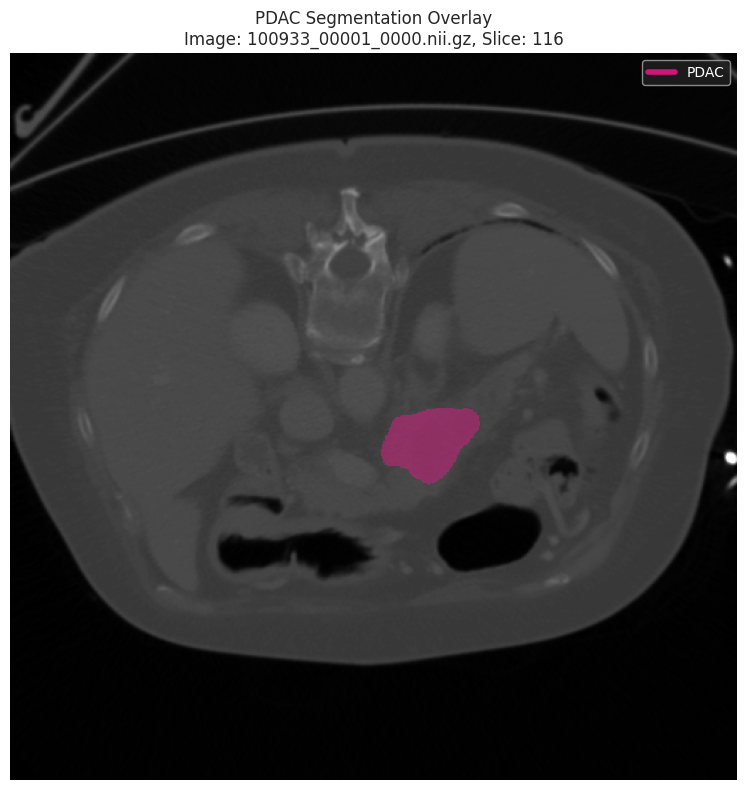
\includegraphics[width=0.75\linewidth]{./figures/pdac_sample.png}
  \caption{A CECT scan slice illustrating Pancreatic Ductal Adenocarcinoma (PDAC).}
  \label{fig:ct_scan}
\end{figure}

Pancreatic ductal adenocarcinoma (PDAC) often leaves only faint radiologic footprints—e.g.\ minimal ductal calibre changes or subtle parenchymal texture shifts—on contrast-enhanced CT (CECT) months before a tumour becomes obvious.  These patterns are easily missed by experts reviewing thousands of abdominal scans for diverse indications.  Modern deep-learning systems, however, thrive on precisely this kind of weak-signal problem: by optimizing millions of parameters across 3-D feature hierarchies, they can amplify and aggregate minute cues that fall below human perceptual thresholds \cite{b7, b8}. See a sample CECT scan from the Grand Challenge dataset in Figure \ref{fig:ct_scan}, marking the lesion location.

The challenge involved over 68 international radiologists and a hidden test cohort of more than 400 cases. The reader study consisted of two components: (1) radiologists provided a binary diagnosis along with a PDAC likelihood score, and (2) for cases identified as PDAC, they marked the lesion location using point annotations. This setup enabled a rigorous comparison between human and algorithmic performance. The \textsc{Panorama} challenge thus provides the first large-scale test bed for PDAC detection systems, with several distinguishing characteristics:

\begin{itemize}[leftmargin=*]
  \item \textbf{Data volume.} Annotated scans of $>$2238 cases for open development.
  \item \textbf{Human baseline.} 68 international radiologists supply a reader-study benchmark, enabling rigorous algorithm-vs-expert comparison.
  \item \textbf{Task design.} Algorithms are evaluated on (i) binary PDAC presence scores and (ii) voxel-level lesion localisation, mirroring real-world deployment needs.
\end{itemize}

State-of-the-art deep learning approaches, such as the PANDA model described by Cao et al. (2023) which utilizes components like CNNs and transformers, have reported NCCT AUCs $>0.95$ for pancreatic lesion detection on single-centre cohorts \cite{b9}. Yet external validation is rare, and most models are tuned on datasets an order of magnitude smaller than \textsc{Panorama}. Critically, these smaller datasets typically have fewer different data sources, leading to lower overall variance between samples, which will likely boost prediction scores but is unlikely to generalize well.

In this project, we aimed to improve upon the winning submission of the \textsc{Panorama} competition [reference to Hiu et al] by focusing on reducing false positives (FP) in the detection of PDAC. We explored a single approach to achieve this: modifying the loss function used during training to incorporate the Tversky loss \cite{b10}, which allows for a more nuanced control over false positive and false negative rates. For example, \cite{Salehi 2017 DOI: 10.1007/978-3-319-67389-9_44} showed that incorporating the Tversky loss in their 3D-UNet model for detecting multiple sclerosis improved the F2 score from $51.77$ to $57.32$, compared to the Dice loss alone. Additionally, reducing FP rates is particularly relevant in medical imaging, where the cost of false positives can lead to unnecessary additional tests and increased workload for radiologists. We also compared to the baseline model, which used a standard cross-entropy loss function [citation], and evaluated the impact of this modification on the area under the ROC curve (AUC) and the Dice score, showing the segmentation performance of the model.

\section{Methods}
This section outlines the methods used to improve the PDAC segmentation model, focusing on the modifications made to the baseline model and the rationale behind these changes. We also elaborate on the dataset used, Tversky loss, and experimentation. 

\subsection{Dataset}
The dataset used in this project is the \textsc{Panorama} dataset, which consists of 2238[check the number] contrast-enhanced computed tomography (CECT) scans annotated by radiologists. The dataset was not split a priori into training and test sets, as the competition organizers had a separate hidden test set for evaluation on the Grand Challenge platform. However, the nnUNet framework trains the models in folds, where each fold is split into training and validation sets anew. Table \ref{tab:presence_pdac} and Figure \ref{fig:pdac_distribution} show the distribution of PDAC presence in the dataset, indicating that the dataset is imbalanced, with a significant number of cases without PDAC.  
\subsection{Baseline Model and nnU-net Framework} 
We chose to use the winning submission of the \textsc{Panorama} competition as a starting point for our own experiment. We considered using the competition baseline but found them to be very similar, with the competition winner's repo being easier to follow. This approach uses nnU-net, \cite{b1} an out of the box neural net solution that builds on the U-net architecture that is specifically tuned for biomedical use cases and is designed to automatically configure itself for optimal performance on a given dataset. Additionally, nnU-net can automatically adapt preprocessing, neural net architecture, and post processing according to the data it is classifying.

The full inference pipeline consists of 4 steps: down-sampling, low-res prediction, masking and high-res prediction. First images are loaded and the voxels are down-sampled according to a set spacing, primarily to manage computational resources and standardize input saves computational cost. Then the nnU-net makes a mask prediction, aiming to identify the rough area of the pancreas. Size-standardized down-sampling save computational cost without losing predictive ability. All hyper-parameters for the prediction were left as the nnU-Net defaults. The mask is represented as a bounding box which is applied to the original image. Finally, a second prediction is made, this time at full resolution but only using the area within the bounding box. This prediction produces two outputs, the full scan of the patient with lesion candidate likelihoods applied to each voxel as well as a single number representing the probability that a patient has a pancreatic lesion. Here the Cross-Entropy is explicitly set for the loss, and the baseline model uses a ResUNet architecture with 3D convolutions.


\section{Improving the Baseline with Tversky Loss}

When considering how to improve the baseline, we explored various potential approaches and evaluated their feasibility. We quickly determined that the most effective objective was to shift the AUC curve to the left. This shift reduces the false positive (FP) rate, thereby decreasing the workload for radiologists and physicians, who must review all cases flagged as positive. [this could be more formal and provide actual reasoning, instead of stating that we had discussions]

One approach we investigated involved training the network using the Tversky loss, a loss function widely adopted in medical image analysis for its ability to handle class imbalance effectively. The Tversky loss quantifies the dissimilarity between the predicted segmentation and the ground truth, and can be viewed as a generalization of the Jaccard index \cite{b3}. It introduces two tunable parameters, $\alpha$ and $\beta$, which allow differential penalization of false positives (FP) and false negatives (FN). Specifically, setting $\alpha > \beta$ increases the penalty on false positives, while $\beta > \alpha$ emphasizes reducing false negatives. This flexibility allows Tversky loss to fine-tune the trade-off between precision and recall, making it particularly useful in scenarios where the cost of false positives and false negatives is not equal. In our case, where minimizing false positives and maximizing precision is crucial, Tversky loss provides an effective way to bias the model accordingly.

\[
\text{TI} = \frac{\text{TP}}{\text{TP} + \alpha \cdot \text{FN} + \beta \cdot \text{FP}}
\]

To integrate the Tversky loss into the nnU-Net framework, we implemented a custom trainer class, [nname], which inherits from the base nnUNetTrainer. This custom trainer was modified to utilize the Tversky loss function, with parameters $\alpha=$ and $\beta=$, for the segmentation task during model training, replacing the default Cross-Entropy loss for this component. Owing to significant computational requirements, the model incorporating Tversky loss was trained and evaluated on a single data fold from the nnU-Net's 5-fold cross-validation scheme. The baseline Cross-Entropy model was trained on all 5 folds for comparison. Performance metrics reported in Section IV for the Tversky model are based on this single fold. For comparative analysis, Receiver Operating Characteristic (ROC) curves were generated for both the baseline and Tversky loss models based on their patient-level PDAC probability scores. Furthermore, qualitative comparisons of segmentation predictions were performed on identical samples from the test set of the evaluated fold.
\section{Results}



\section{Conclusions}
When building any machine learning models for medical applications, it is important to consider not only the performance metrics such as accuracy or $F_1$ score but also the practical implications of false positives and false negatives. In this project, we focused on reducing false positives in the detection of pancreatic ductal adenocarcinoma (PDAC) by modifying the loss function used during training to incorporate the Tversky loss. This approach allowed us to fine-tune the trade-off between false positives and false negatives, which is particularly relevant in medical imaging where the cost of false positives can lead to unnecessary additional tests and increased workload for radiologists.

We implemented a custom trainer class in the nnU-Net framework to utilize the Tversky loss function, and trained the model on a single fold of the \textsc{Panorama} dataset. The results showed that the Tversky loss model achieved a [performance] area under the ROC curve (AUC) compared to the baseline model using cross-entropy loss, indicating [...] performance in reducing false positives. Additionally, qualitative comparisons of segmentation predictions demonstrated that the Tversky loss model produced [....] accurate segmentations of PDAC lesions.

Our findings are in line with previous studies that have shown the effectiveness of Tversky loss in improving segmentation performance in medical imaging tasks. However, yet alone, the Tversky loss may not be optimimal for decreasing false positives, and other its variations tend to be more effective, such as the Focal Tversky loss \cite{b3}. Future work could explore the use of Focal Tversky loss or other variations to further improve the model's performance in reducing false positives. Additionally, we could also consider incorporating attention mechanisms or other advanced techniques to enhance the model's ability to focus on relevant features in the CECT scans.



\begin{thebibliography}{00}
\bibitem{b1} Isensee, F., Jaeger, P.F., Kohl, S.A.A. et al. nnU-Net: a self-configuring method for deep learning-based biomedical image segmentation. Nat Methods 18, 203–211 (2021). https://doi.org/10.1038/s41592-020-01008-z
\bibitem{b2} National Cancer Institute, ``SEER Cancer Stat Facts: Pancreatic Cancer,'' https://seer.cancer.gov/statfacts/html/pancreas.html, accessed May 15, 2025.
\bibitem{b3} Saba, M., ``Tversky Loss,'' *Medium*, https://medium.com/@saba99/tversky-loss-902f5f8cc35f, accessed May 15, 2025.
\bibitem{b5} PANORAMA Grand Challenge, ``PANORAMA: AI Grand Challenge for Pancreatic Cancer Detection,'' https://panorama.grand-challenge.org/, accessed May 15, 2025.
\bibitem{b6} The Radiology Assistant, ``Pancreas - Carcinoma,'' https://radiologyassistant.nl/abdomen/pancreas/pancreas-carcinoma-1, accessed May 15, 2025.
\bibitem{b7} A. Esteva, B. Kuprel, R. A. Novoa, J. Ko, S. M. Swetter, H. M. Blau, and S. Thrun, ``Dermatologist-level classification of skin cancer with deep neural networks,'' \textit{Nature}, vol. 542, no. 7639, pp. 115--118, 2017, doi: 10.1038/nature21056.

\bibitem{b8} S. M. McKinney, M. Sieniek, V. Godbole, J. Godwin, N. Antropova, H. Ashrafian, T. Back, A. Chesus, D. C. Corrado, B. Darzi, \textit{et al.}, ``International evaluation of an AI system for breast cancer screening,'' \textit{Nature}, vol. 577, no. 7788, pp. 89--94, 2020, doi: 10.1038/s41586-019-1799-6.

\bibitem{b9} K. Cao, Y. Xia, J. Yao, H. Xu, L. Lambert, T. Zhang, W. Tang, G. Jin, J. Hui, F. Xu, I. Nogues, X. Li, W. Guo, Y. Wang, W. Fang, M. Qiu, Y. Hou, T. Kovarnik, M. Vocka, Y. Lu, Y. Chen, X. Chen, Z. Liu, Z. Chen, C. Xie, R. Zhang, H. Lu, G. Hager, A. L. Yuille, L. Lu, C. Shao, Y. Shi, T. Liang, L. Zhang, and J. Lu, ``Large-scale pancreatic cancer detection via non-contrast CT and deep learning,'' \textit{Nature Medicine}, vol. 29, no. 12, pp. 3033--3043, 2023, doi: 10.1038/s41591-023-02640-w.




\bibitem{b10} Salehi, S.S.M., Erdogmus, D., Gholipour, A. (2017). Tversky Loss Function for Image Segmentation Using 3D Fully Convolutional Deep Networks. In: Wang, Q., Shi, Y., Suk, HI., Suzuki, K. (eds) Machine Learning in Medical Imaging. MLMI 2017. Lecture Notes in Computer Science(), vol 10541. Springer, Cham. https://doi.org/10.1007/978-3-319-67389-9_44


\end{thebibliography}
\end{document}
